\section*{Figures}

\begin{figure}[ht]
  \caption{\textbf{Opinion measurement model and spurious group polarization.} 
  Latent model participant opinions are drawn from a normal distribution with the
  listed parameters (A,C). The pre-deliberation latent distribution has high
  variance, but appears polarized when measured via integration (A).  The latent
  distribution's variance is expected to decrease during deliberation (B) via
  consensus, but in this example the latent mean is static, 
$\mupre = \mupost$. However, when the post-deliberation distribution is measured,
the simulated observed mean increases, i.e., spurious
group polarization occurs (C).}
  \centering
  \includegraphics[width=0.95\textwidth]{Figures/Model/latent-ordinal-distros.pdf}
  \label{fig:distros}
\end{figure}


\begin{figure}
    \centering{
    	\includegraphics[width=0.8\textwidth]{Figures/Model/SoftwareMap_Mashup.png}
    }
    
    \caption{\textbf{Computational system to
    interactively simulate opinion change, identify invalid replications,
    and evaluate experimental designs.}}
    \label{fig:computational-system}
\end{figure}


\begin{figure}
  \centering
    % \includegraphics[width=0.8\textwidth]{Figures/Model/data-model-flow.png}
  \includegraphics[width=\textwidth]{Figures/Model/SoftwareMap_Mashup.png}
  \caption{\textbf{Simulation and analysis pipeline}
  for finding when measurement artifacts.  
  Arrows show the flow of input and output data from parameter estimation.
  First, we used the web app (A) to find null-polarization parameters for 
  each experimental condition, $\nu_e$,
  that ordinal measurements distort to look like polarization
  (B—described in Algorithm~\ref{alg:hillclimbing}).
  We fit ordered probit models to simulated null-polarization outcomes,
  seeded by the $\nu$ found in the previous step (C). Analysis and 
  visualization routines finish the pipeline (D).}
  \label{fig:data-model-flow}
\end{figure}



\begin{figure}

  \caption{\textbf{Family-wise error rates and false discovery rates across studies and experiments for
    low, medium, and high Cohen's $d$ significance.}}
  \label{fig:fwer_fdr_synthesis}

  \centering
  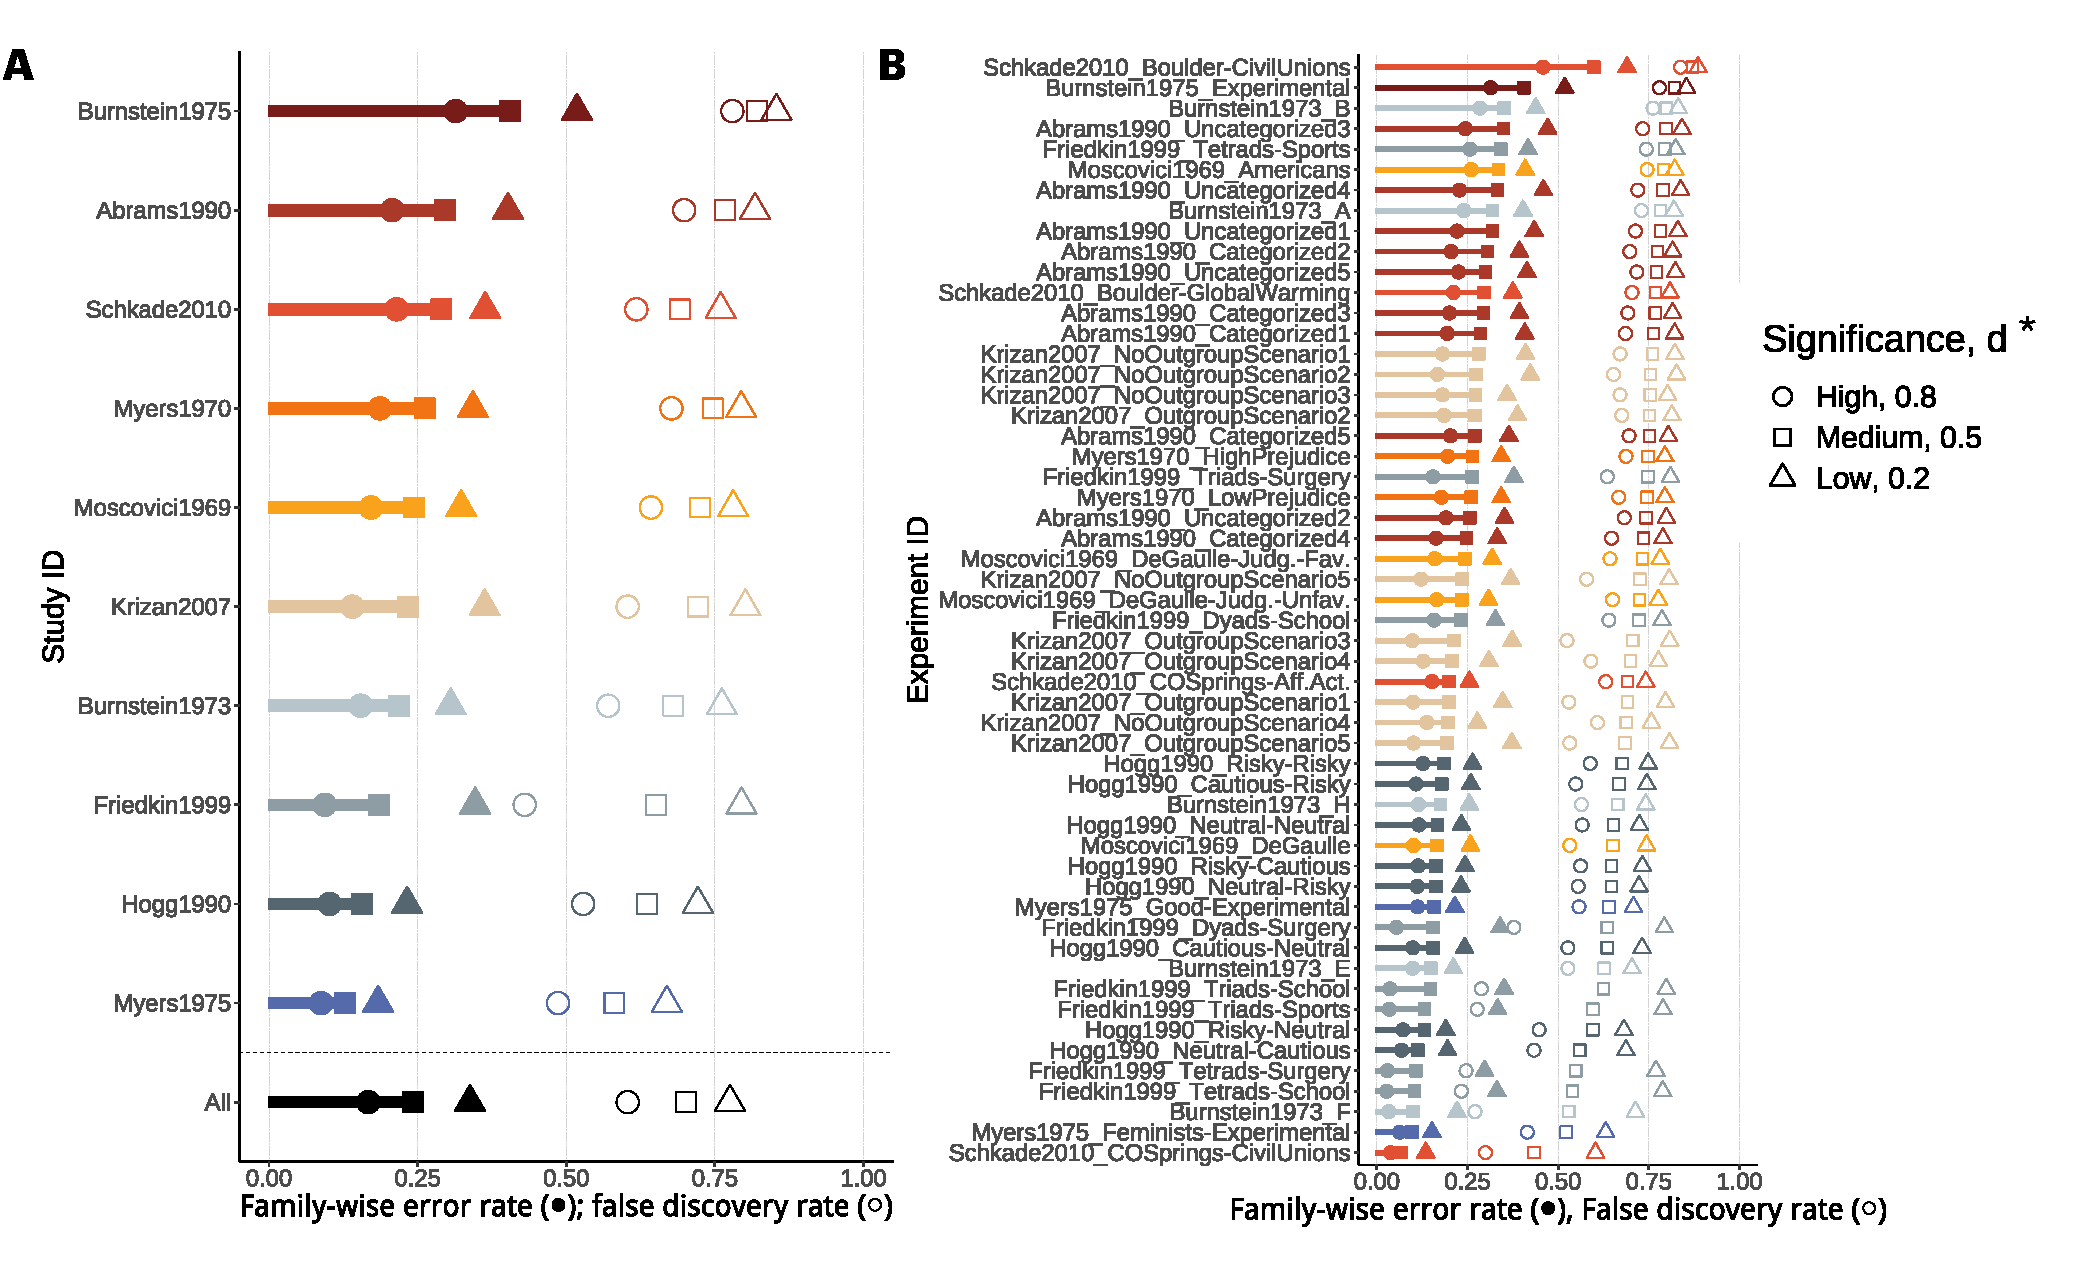
\includegraphics[width=1.1\textwidth]{Figures/Analysis/fwer_fdr_synthesis.pdf}
\end{figure} 


\begin{figure}
  \caption{
    \textbf{Significance value, $d^*$, to limit family-wise error 
    rate of 0.05 for each identified study.} The Moscovici and Zavalloni (1969)
    ``Americans'' question would require the greatest $d^*$ to achieve $\alpha \leq
    0.05$, even though it does not have the highest error rates. This is because of
    larger outliers in simulated $d$ for this condition compared to others with
    greater error rates (Figure~\ref{fig:OrdinalBoxplot}).
  }
  \centering
    \includegraphics[width=0.75\textwidth]{Figures/Analysis/sigval_for_low_fwer.pdf}
  \label{fig:sigval_for_low_fwer}
\end{figure}
